\documentclass[fontset=ubuntu]{ctexart}

% \usepackage{ctex}
\usepackage{graphicx} % 图片
\usepackage{subfigure} %子图片
\usepackage{minted} % 代码
\usepackage{listings} % 代码
\usepackage{enumerate} % 有序列表
\usepackage{float} % 设置位置
\usepackage{hyperref} % 网页链接
\usepackage{fancyhdr} % 页眉页脚

\title{\Huge \textbf{实验报告二 \\ Shell\&Vim\&数据整理}}
\author{\textit{潘奕霖}}
\date{https://github.com/PYL1024/system-develop-tools\\ \today}
\pagestyle{fancy}

\fancyhead{}
\fancyhead[R]{\textsl{\leftmark}}
\fancyfoot{}
\fancyfoot[L]{https://github.com/PYL1024/system-develop-tools}
\fancyfoot[R]{\thepage}
\setlength{\headheight}{14pt}
\addtolength{\topmargin}{-5pt}

\begin{document}
\begin{sloppypar}

\maketitle
\newpage

\tableofcontents
\newpage

\section{shell学习感悟}
要在Windows上拥有接近原生Linux系统的shell使用体验,我认为wsl是最快捷的选择。不需要像虚拟机一样下载镜像,再经过漫长的安装过程,只需要一些前置步骤,再使用几行命令,就可以获得几乎完美的使用体验,并且可以与Windows系统互通文件,十分方便。

shell的上手难度并不算大,掌握mkdir,cd,ls,touch,mv,rm,vim的基本用法,就基本上能满足日常的使用需要,而且有man,tldr这样快捷的帮助工具,帮助你获取某个命令的用法。而且Linux下有许多极具特色的小工具,能简化或是增强原有的shell操作,对这些小工具的灵活使用能大大增强使用shell的效率和幸福感。

自定义shell也是个人认为比较重要的,可以为其安装主题和插件,来显示更多信息与提供自动补全命令的功能,提升使用的效率。

不过shell的进阶操作还是有一些学习成本,毕竟命令行界面没有图形界面那么直观,有时还会出现莫名其妙的bug。Linux上的某些操作还需要格外谨慎,用\mintinline{shell}|mv|删错东西可没有后悔药可吃,移动错文件位置有时找半天找不回来,这些都是使用时要格外避免的。

注意自己写的脚本文件和Python文件需要添加执行权限才能运行。

\section{shell知识点}
\subsection{基本操作}
\subsubsection{创建文件夹}
创建文件夹:\mintinline{shell}|mkdir|
\begin{figure}[htb]
    \centering
    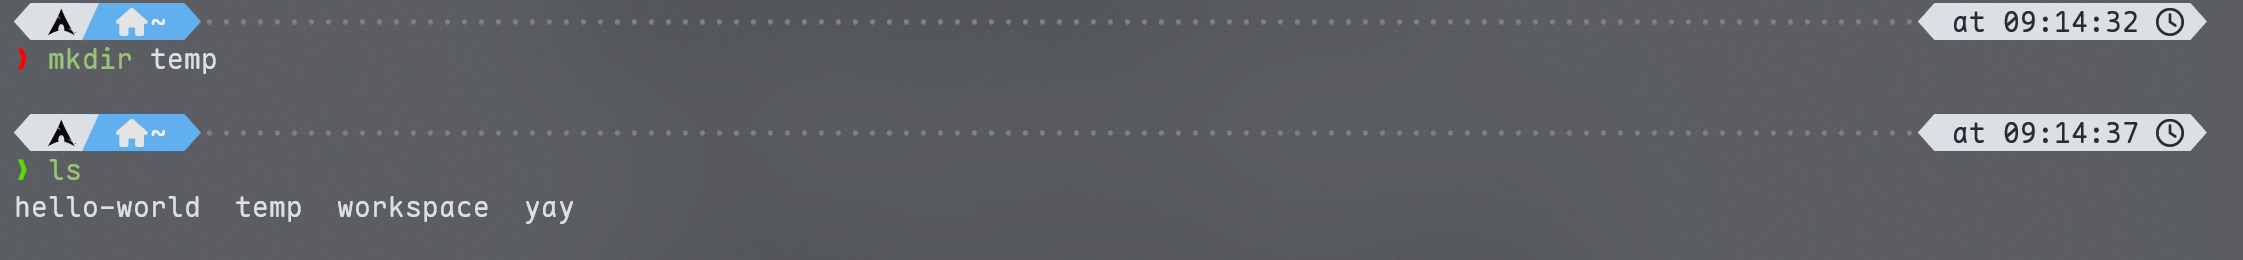
\includegraphics[width=0.75\linewidth]{mkdir_1.png}
    \caption{mkdir}
    \label{fig:mkdir_1}
\end{figure}

-m参数后接rwx等,可以同时设定文件夹的权限。

\subsubsection{创建文件}
创建文件:\mintinline{shell}|touch|
\begin{figure}
    \centering
    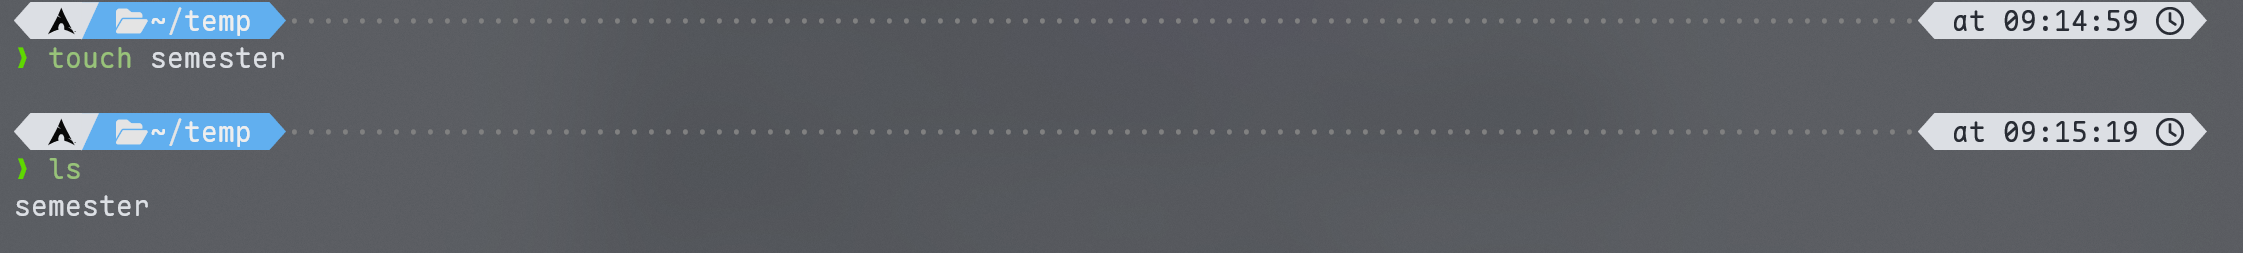
\includegraphics[width=0.75\linewidth]{touch_1.png}
    \caption{touch}
    \label{fig:touch_1}
\end{figure}

\mintinline{shell}|touch|还有设定文件修改时间和文件时间戳的功能。

\subsubsection{列出文件夹下的文件}
列出文件:\mintinline{shell}|ls|
\begin{figure}[htb]
    \centering
    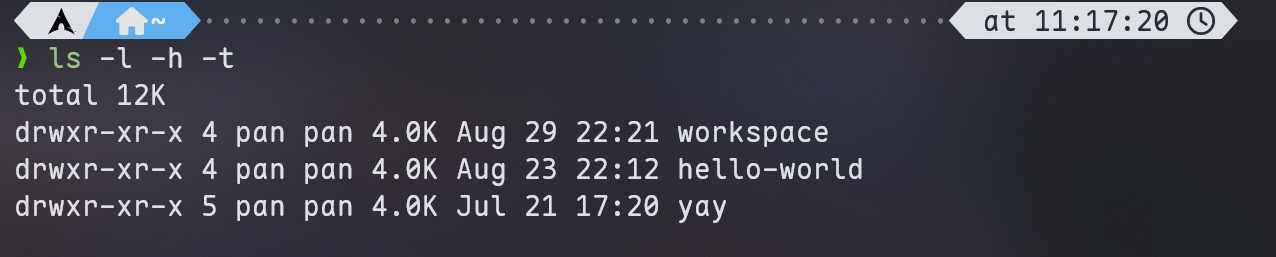
\includegraphics[width=0.75\linewidth]{ls_1.png}
    \caption{ls}
    \label{fig:ls_1}
\end{figure}

不加参数仅会列出文件名,-lh以利于人类理解的方式输出,即以M或K为单位,--color=auto自动通过颜色区分文件和目录,--block-size=K将文件单位设为K,也可设为M。

\subsubsection{打印内容}
打印内容:\mintinline{shell}|echo|
\begin{figure}[htb]
    \centering
    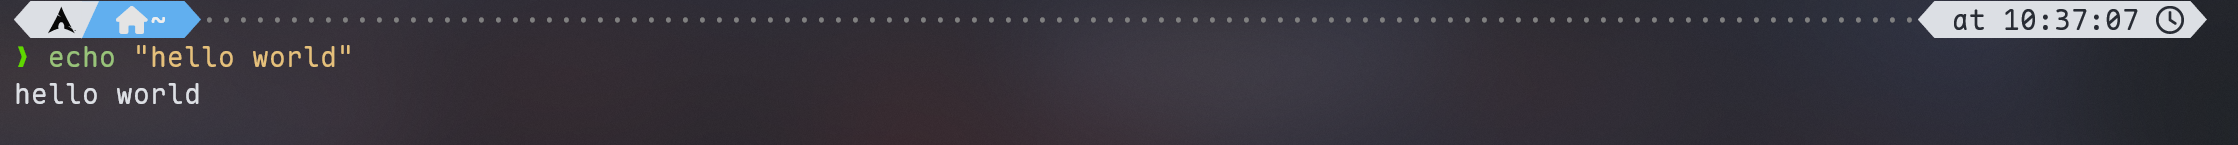
\includegraphics[width=0.75\linewidth]{echo_1.png}
    \caption{echo}
    \label{fig:echo_1}
\end{figure}

\mintinline{shell}|echo|可以打印纯文本,也可以配合\$与shell中的变量名打印信息,还可以与重定向操作符配合向文件中写入信息。
\begin{figure}[htb]
    \centering
    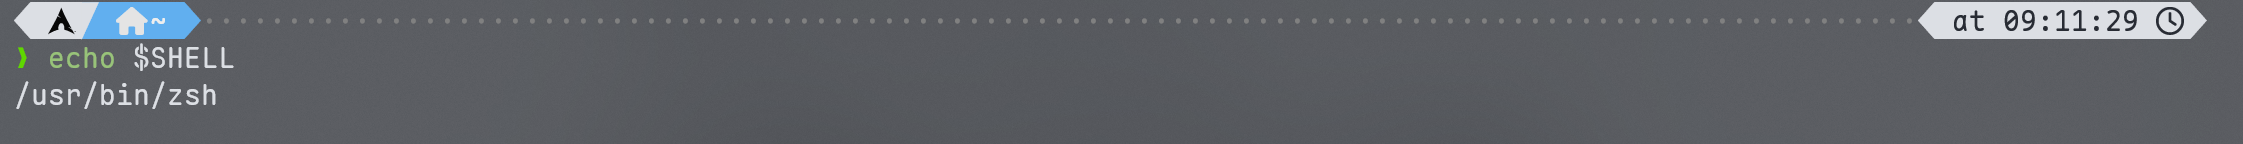
\includegraphics[width=0.75\linewidth]{shell_1.png}
    \caption{显示当前的shell}
    \label{fig:shell_1}
\end{figure}

\subsubsection{修改权限}
修改权限:\mintinline{shell}|chmod <-cfvR> <filename>|
\begin{figure}[htb]
    \centering
    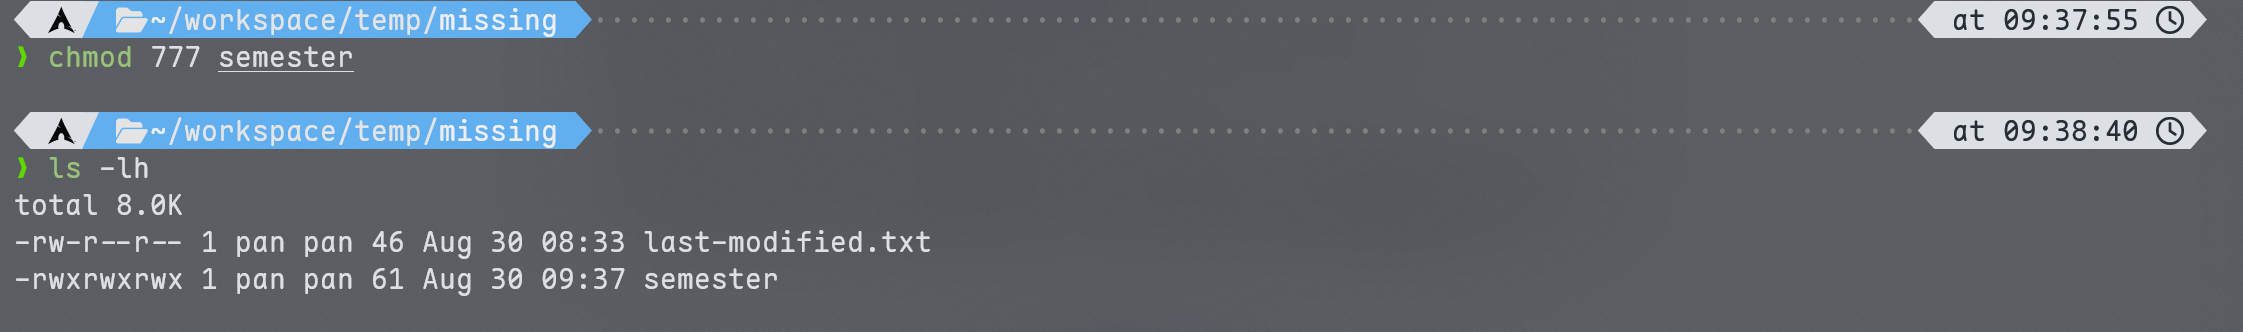
\includegraphics[width=0.75\linewidth]{chmod_1.png}
    \caption{chmod}
    \label{fig:chmod_1}
\end{figure}

权限的授予对象有owner,group,other,只有owner和root用户可以修改权限。权限命令的格式有两大类:符号模式和八进制语法。符号模式使用u,g,o代表三个群体,+,-代表增加或减少权限,w,r,x代表写、读、执行三个权限,可以组成命令如u+x。八进制语法即以4,2,1代表读、写、执行,使用\mintinline{shell}|chmod 777|可以为所有用户赋予权限。

\subsubsection{查看命令用法}
查看用法:\mintinline{shell}|man <command>|
\begin{figure}[htb]
    \centering
    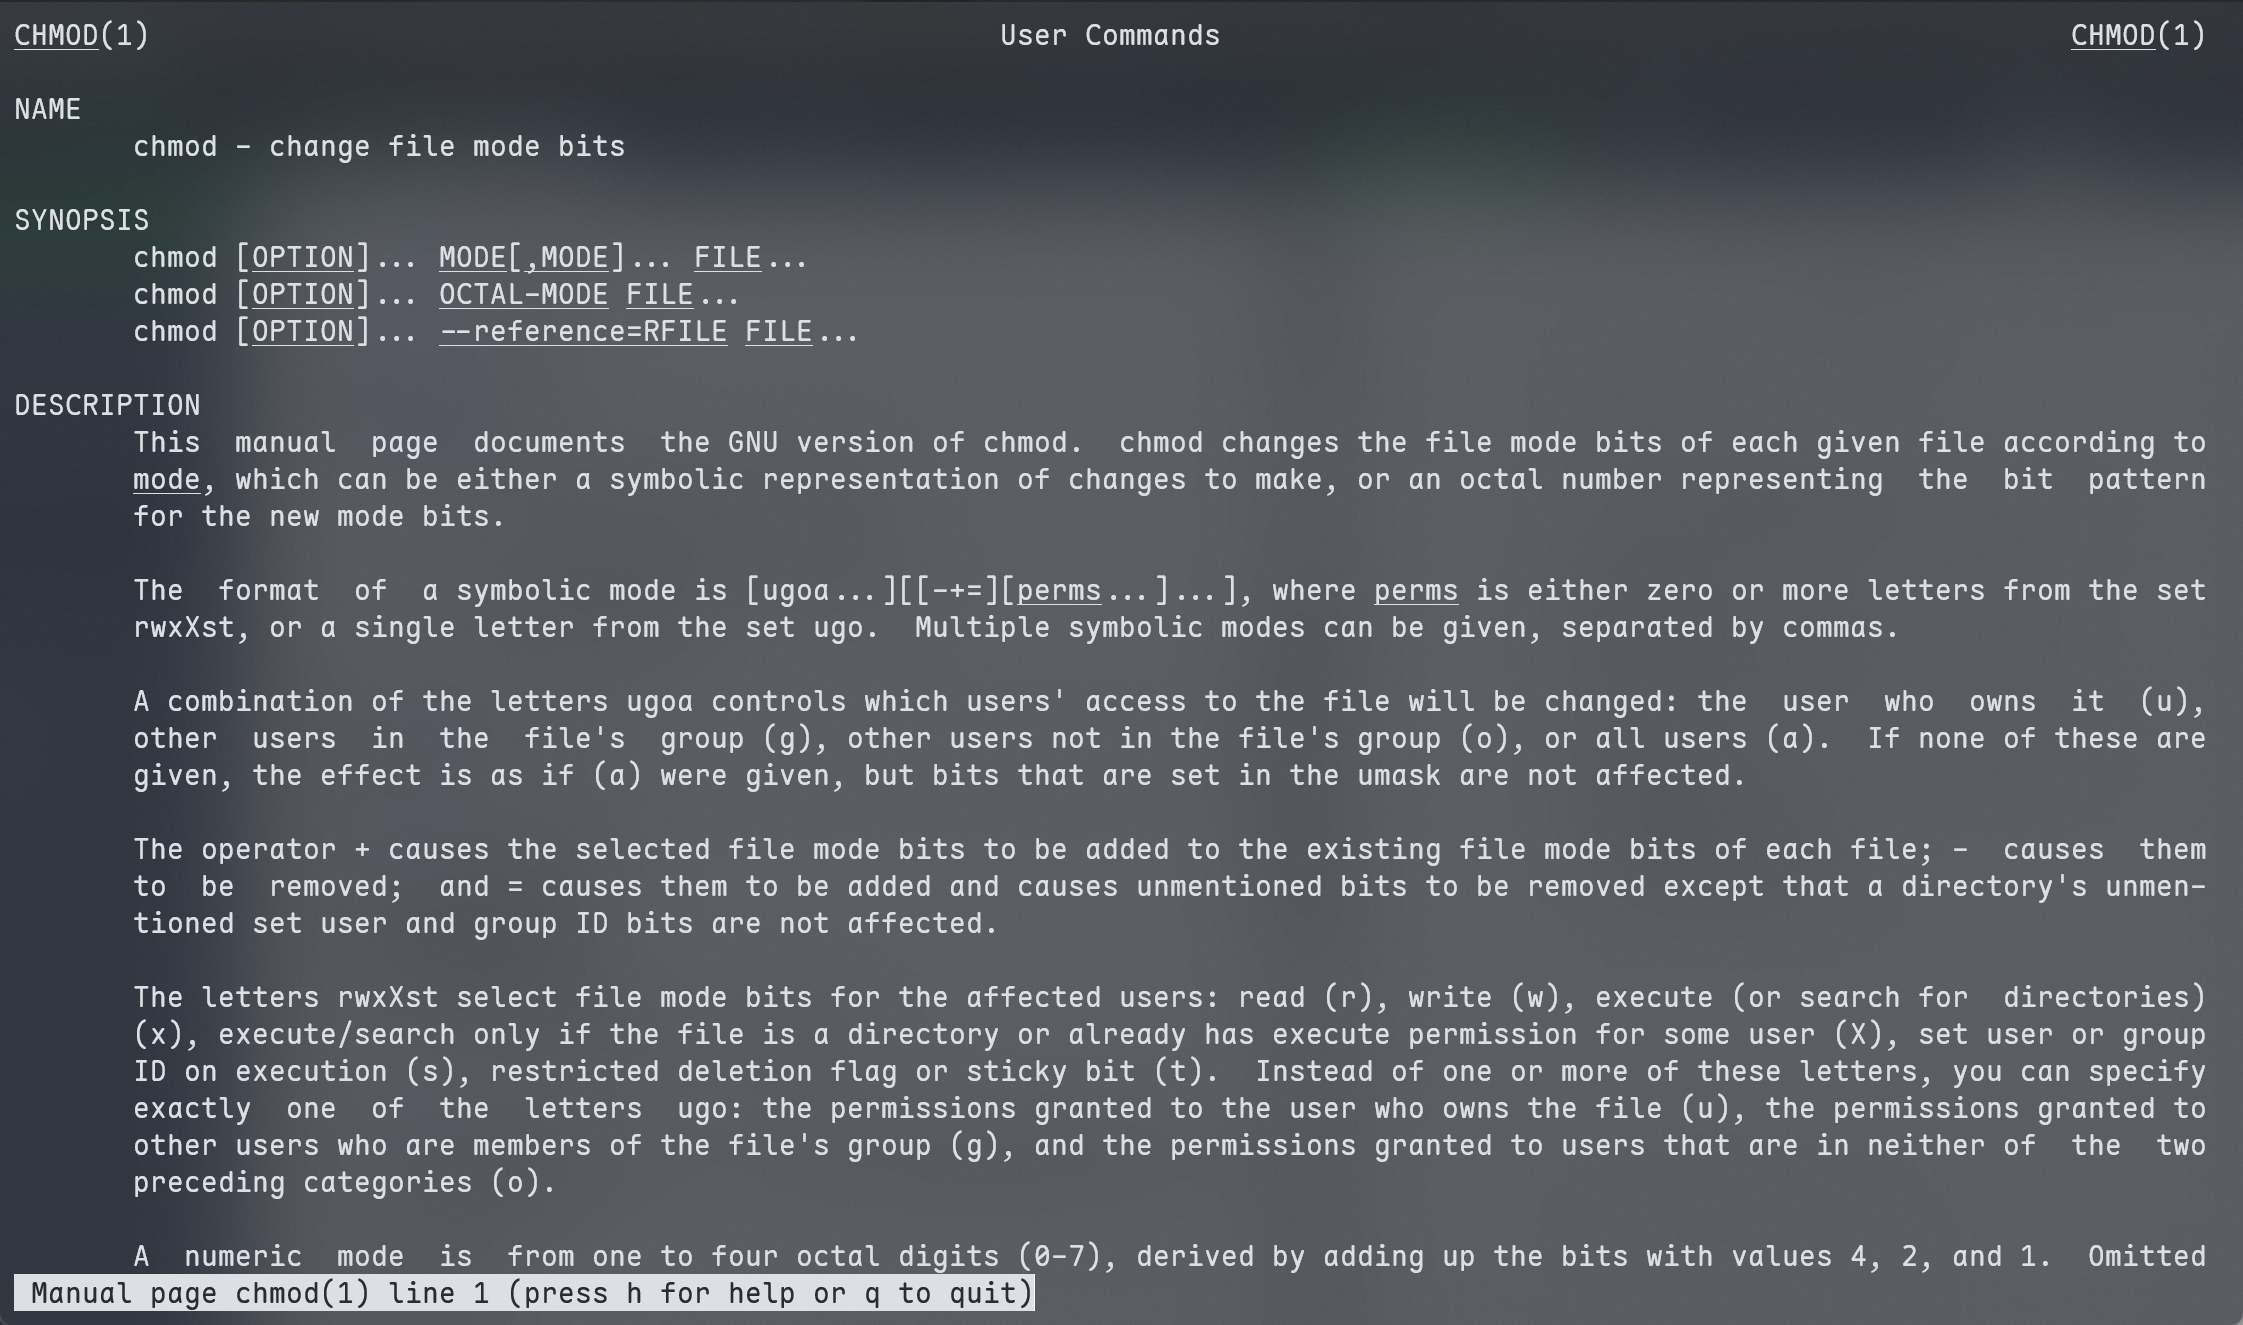
\includegraphics[width=0.75\linewidth]{man_1.png}
    \caption{man}
    \label{fig:man_1}
\end{figure}

man也有替代品,比如tldr。tldr是Too Long; Didn’t Read的缩写,能够提供更加简洁的提示和说明。使用\mintinline{shell}|sudo pacman -S tldr|安装tldr,在安装完成后要先\mintinline{shell}|tldr -u|加载缓存,再输入查询命令。
\begin{figure}[htb]
    \centering
    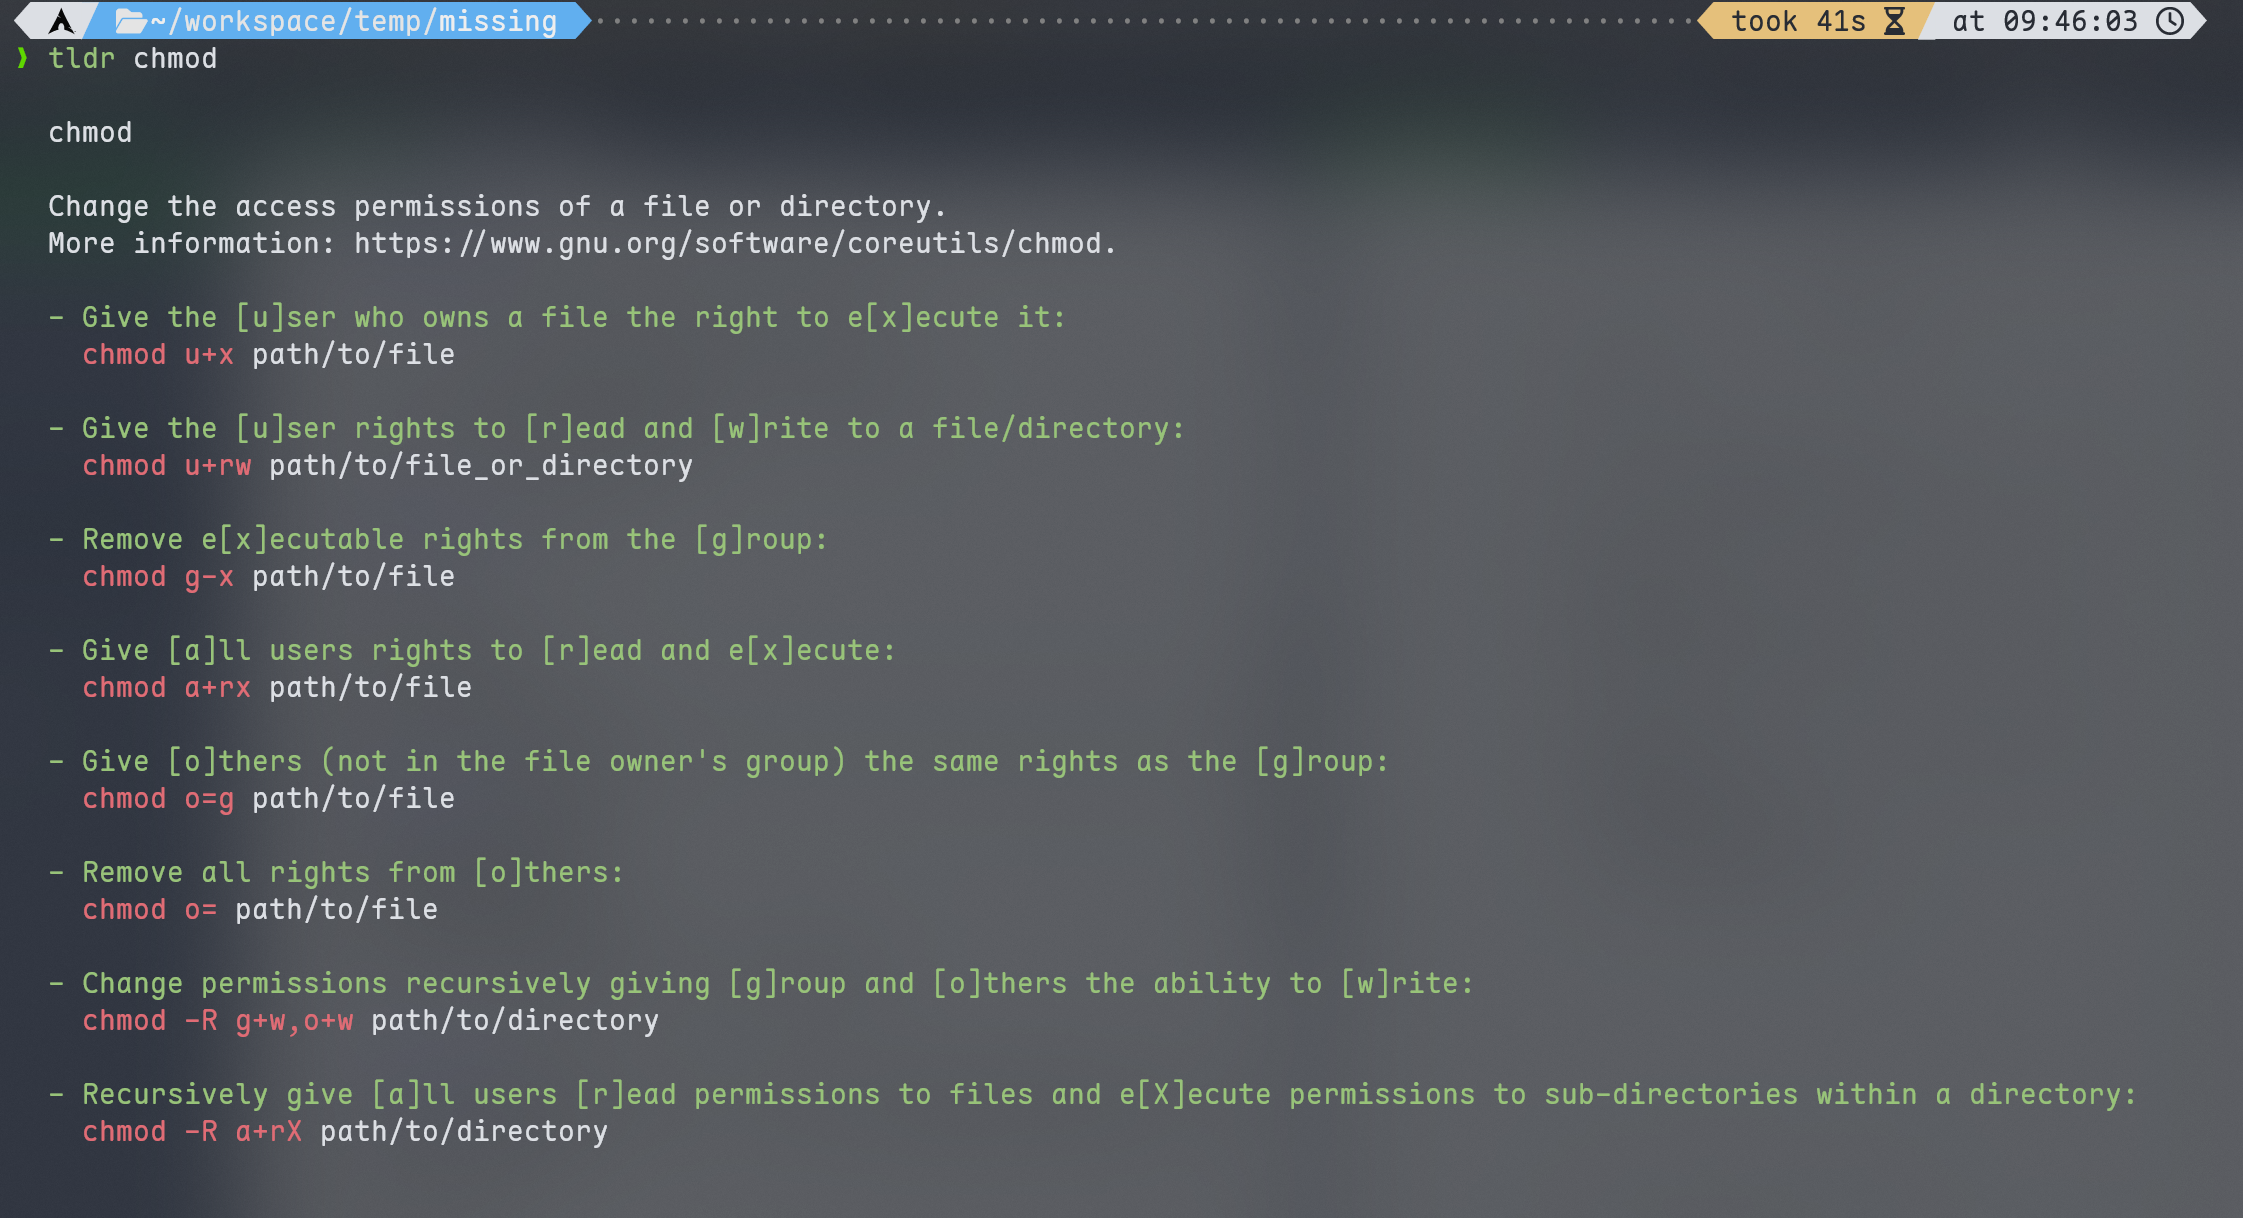
\includegraphics[width=0.75\linewidth]{tldr_1.png}
    \caption{tldr}
    \label{fig:tldr_1}
\end{figure}

\subsection{向文件内写入具有特殊含义的字符}
配合使用\mintinline{shell}|echo > >> ' '|能将具有特殊含义的字符写入文件中。比如将\#!/bin/sh写入文件,由于\#和\!在shell中有特殊含义,需要使用\mintinline{shell}|' '|包裹整个语句,再使用\mintinline{shell}|>|将输出重定向至文件。这里要注意\mintinline{shell}|> >>|的区别,前者会将文件内容清空再进行写入,而后者是进行追加。同时要注意\mintinline{shell}|' ' " "|的区别,单引号仅保留其中字符的文字意义,而双引号会使其中的特殊字符产生特殊意义,借助这一点可以在\mintinline{shell}|echo|语句中一同输出某些变量的值。
\begin{figure}[htb]
    \centering
    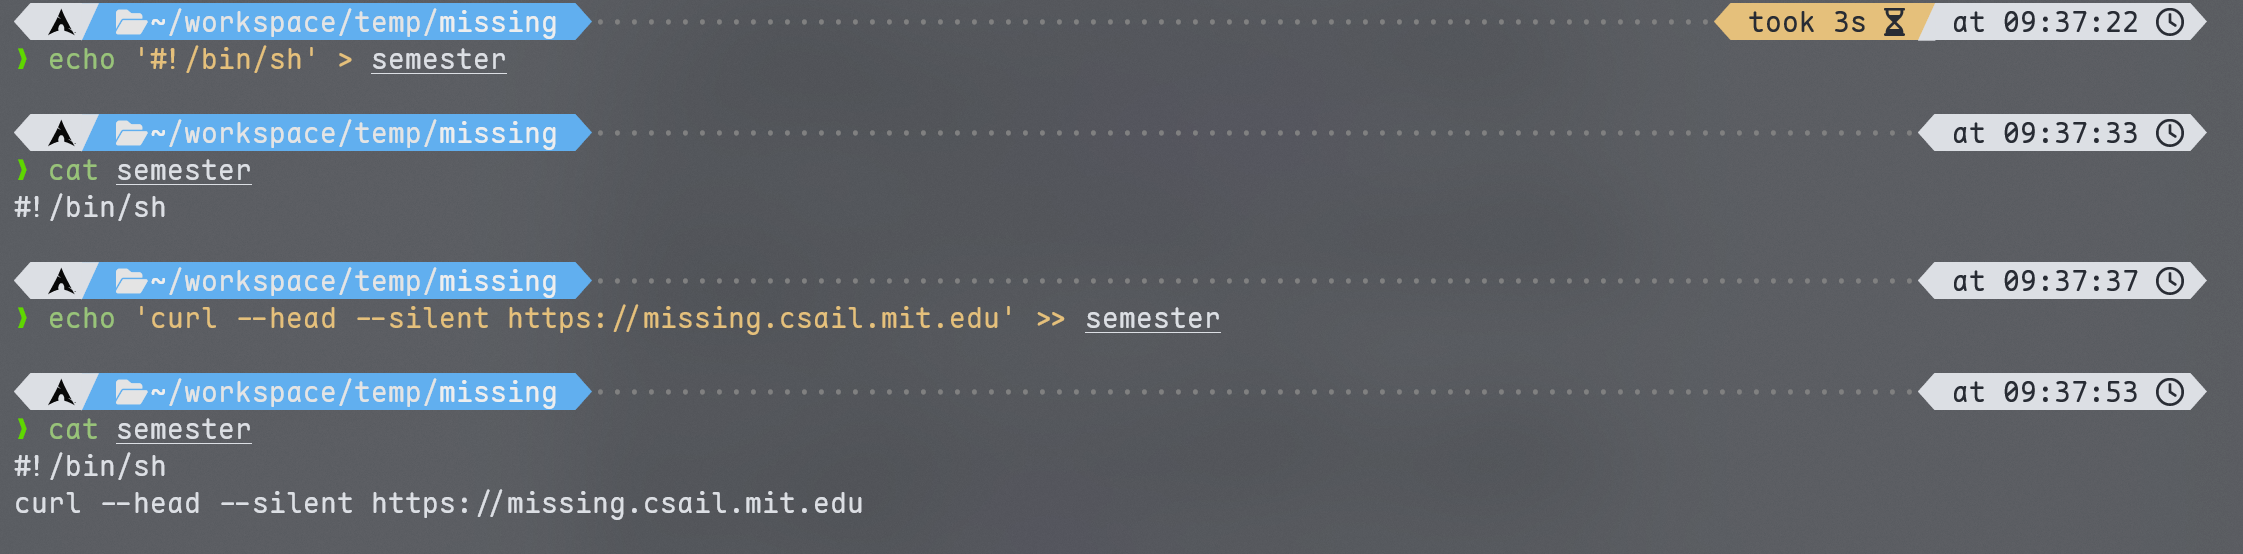
\includegraphics[width=0.75\linewidth]{to_file_1.png}
    \caption{向文件写入特殊字符}
    \label{fig:to_file_1}
\end{figure}

注意\mintinline{shell}|2>|代表错误输出,后面接\mintinline{shell}|&1|能将错误输出重定向到标准输出。如\mint{shell}|command >> file 2>&1|

不需要的输出可以重定向至/dev/null,所有写入的内容都会被抛弃。

\subsection{输出文件内容}
输出文件内容:\mintinline{shell}|cat|,能将文件内容输出到标准输出流,也可以配合重定向操作符将结果输出到文件,以下是使用\mintinline{shell}|cat|查看电池电量的操作:
\begin{figure}[htb]
    \centering
    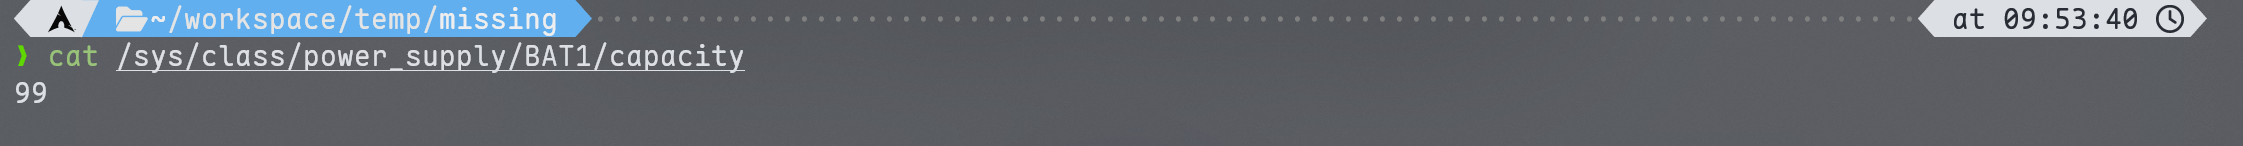
\includegraphics[width=0.75\linewidth]{cat_1.png}
    \caption{cat}
    \label{fig:cat_1}
\end{figure}

\subsection{在文件或输出流中搜索}
搜索字符串:\mintinline{shell}|grep|,能在文件或输出流中搜寻匹配的字符串,十分好用的寻找工具,配合管道和重定向就能将搜寻到内容保存到文件。如将semester脚本输出的某一特定行存入文件。
\begin{figure}[htb]
    \centering
    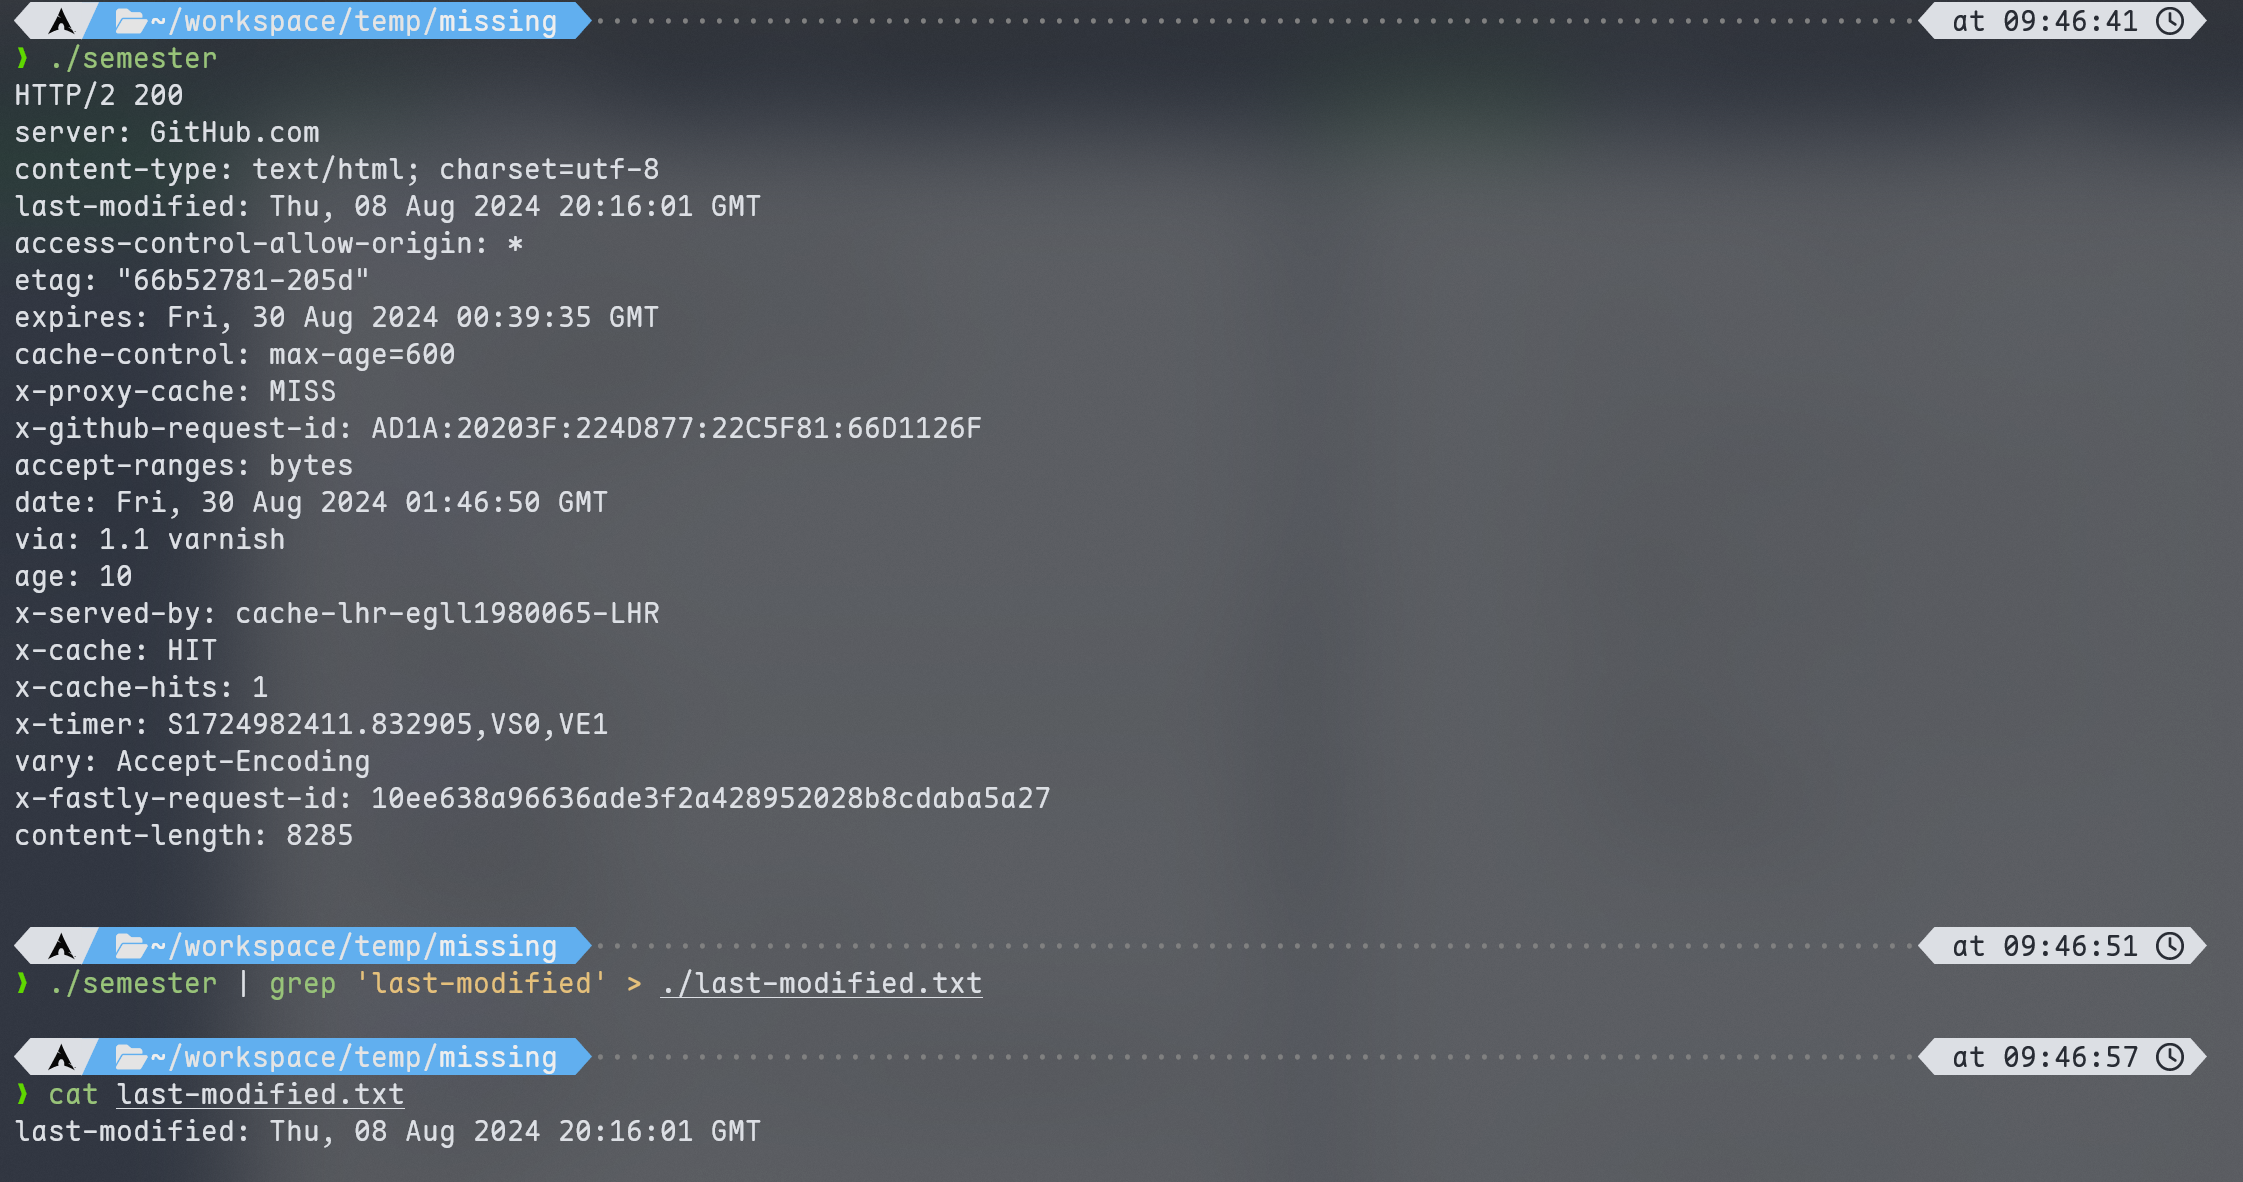
\includegraphics[width=0.75\linewidth]{grep_1.png}
    \caption{grep}
    \label{fig:grep_1}
\end{figure}

\subsection{搜索文件}
搜索文件:\mintinline{shell}|find|,能够依据拓展名,大小,修改时间等一系列条件搜索文件,效率很高。
\begin{figure}[htb]
    \centering
    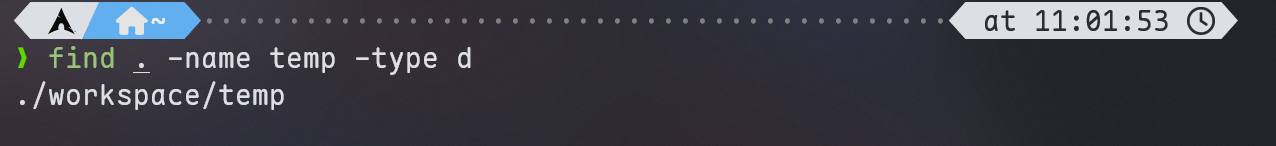
\includegraphics[width=0.75\linewidth]{find_name_1.png}
    \caption{根据名称搜索}
    \label{fig:find_name_1}
\end{figure}

\begin{figure}[htb]
    \centering
    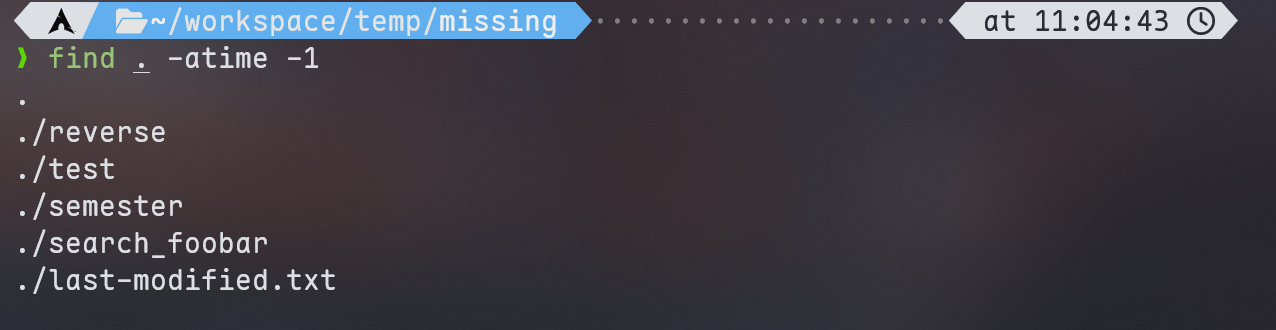
\includegraphics[width=0.75\linewidth]{find_time_1.png}
    \caption{根据修改时间搜索}
    \label{fig:find_time_1}
\end{figure}

\subsection{定义函数}
在shell中也可以直接定义函数,不写入文件。输入函数名和(),回车,会出现
\mintinline{shell}|function>|,若是定义多行函数需要输入{},否则回车后就会退出函数定义。
在shell中定义了mcd函数,可以在创建文件夹后进入该文件夹。这样定义的函数在退出shell后就会被销毁。
\begin{figure}[htb]
    \centering
    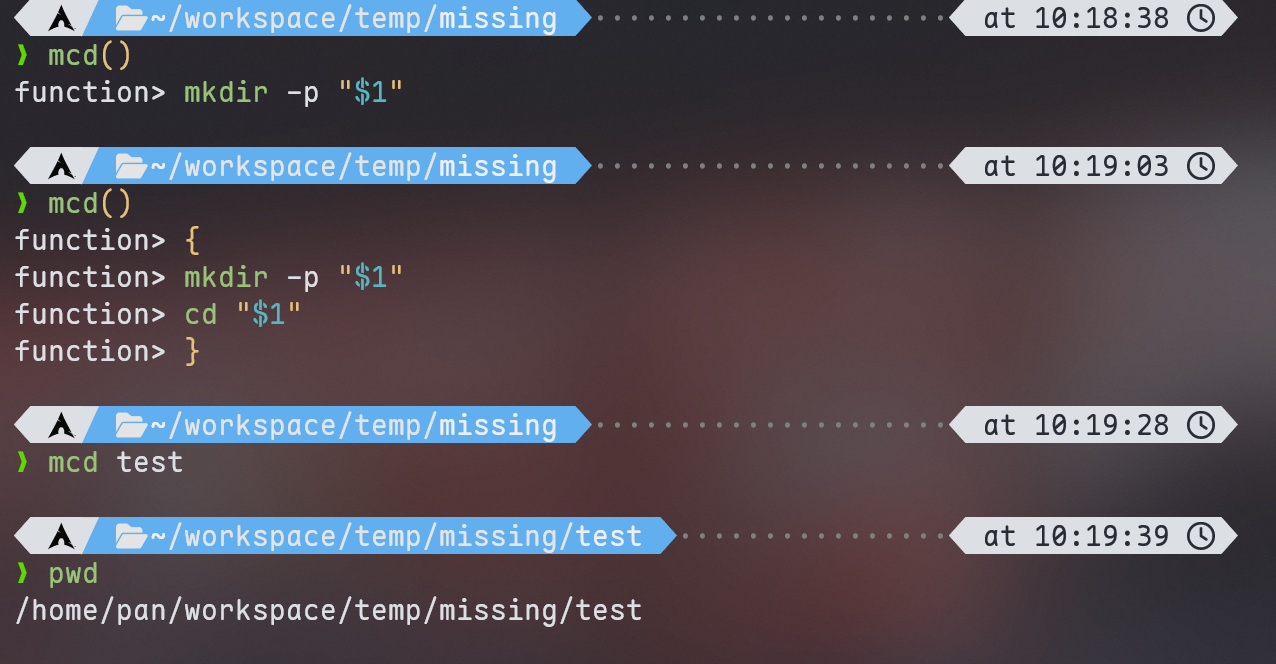
\includegraphics[width=0.75\linewidth]{function_1.png}
    \caption{function}
    \label{fig:function_1}
\end{figure}

\subsection{shell中的特殊变量}
\begin{itemize}
    \item \$0:脚本名
    \item \$1-\$9:脚本的参数
    \item \$@:所有参数
    \item \$\#:参数个数
    \item \$?:前一个命令的返回值
    \item \$\$:当前脚本的进程识别码
\end{itemize}

\subsection{记录所在目录并能快速前往的脚本}
marco脚本中的\mintinline{shell}|export|将MARCO移动到子进程,\verb|$|能用命令的输出结果替换\verb|$|语句,即将当前所在的路径存进了MARCO变量。polo脚本则获取MARCO变量的值,再切换到这个目录。
\begin{figure}[htb]
    \centering
    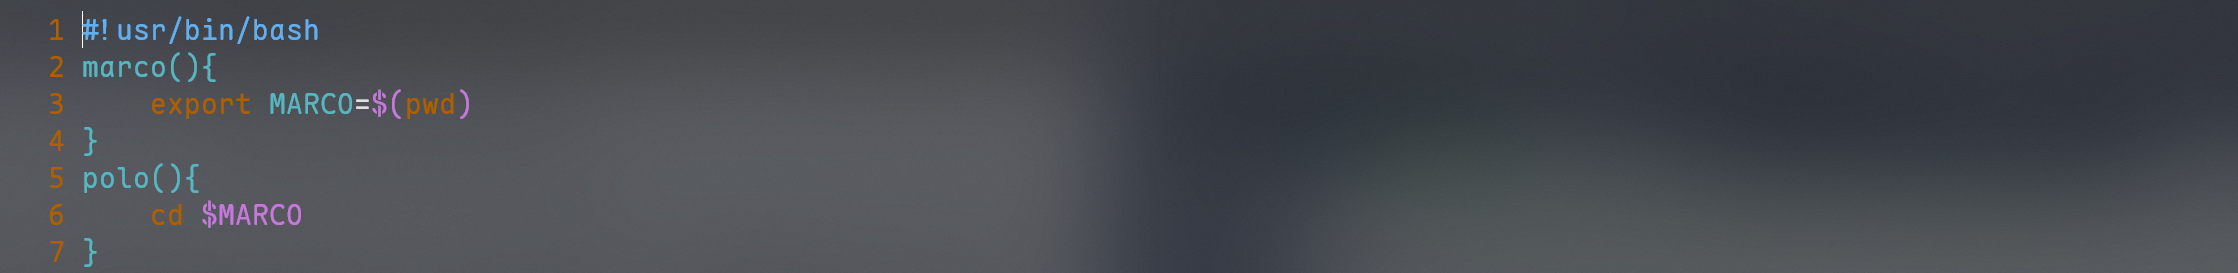
\includegraphics[width=0.75\linewidth]{marco_1.png}
    \caption{脚本内容}
    \label{fig:marco_1}
\end{figure}

\begin{figure}[htb]
    \centering
    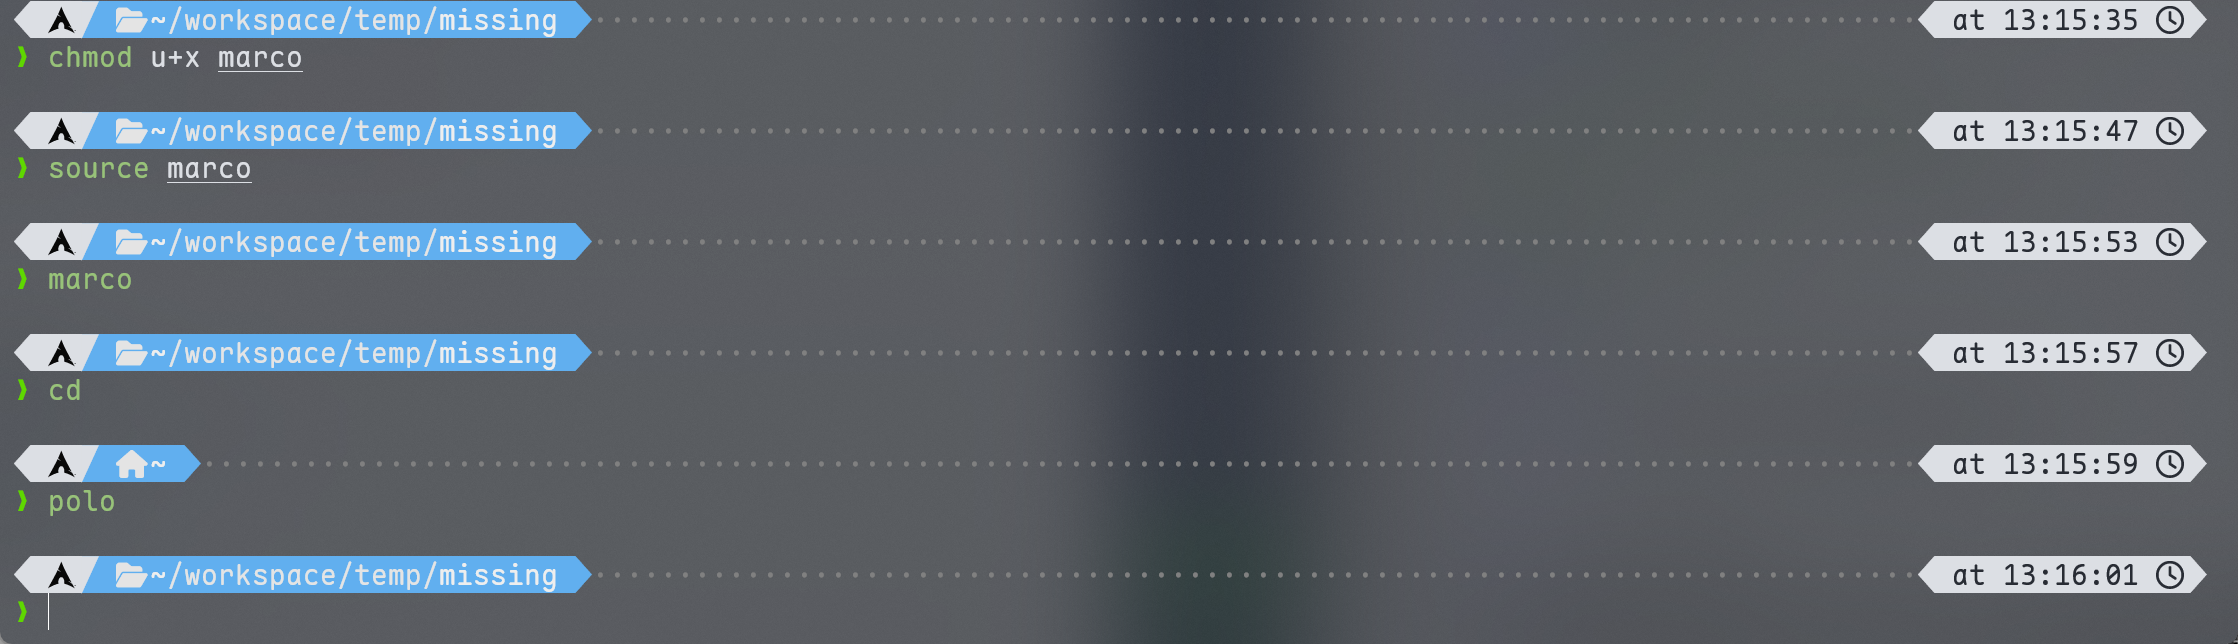
\includegraphics[width=0.75\linewidth]{polo_1.png}
    \caption{脚本效果}
    \label{fig:polo_1}
\end{figure}

\subsection{记录某一脚本运行次数}
用for循环,每循环一次进行一次计数,要注意shell语言的特殊符号。
\begin{figure}[htb]
    \centering
    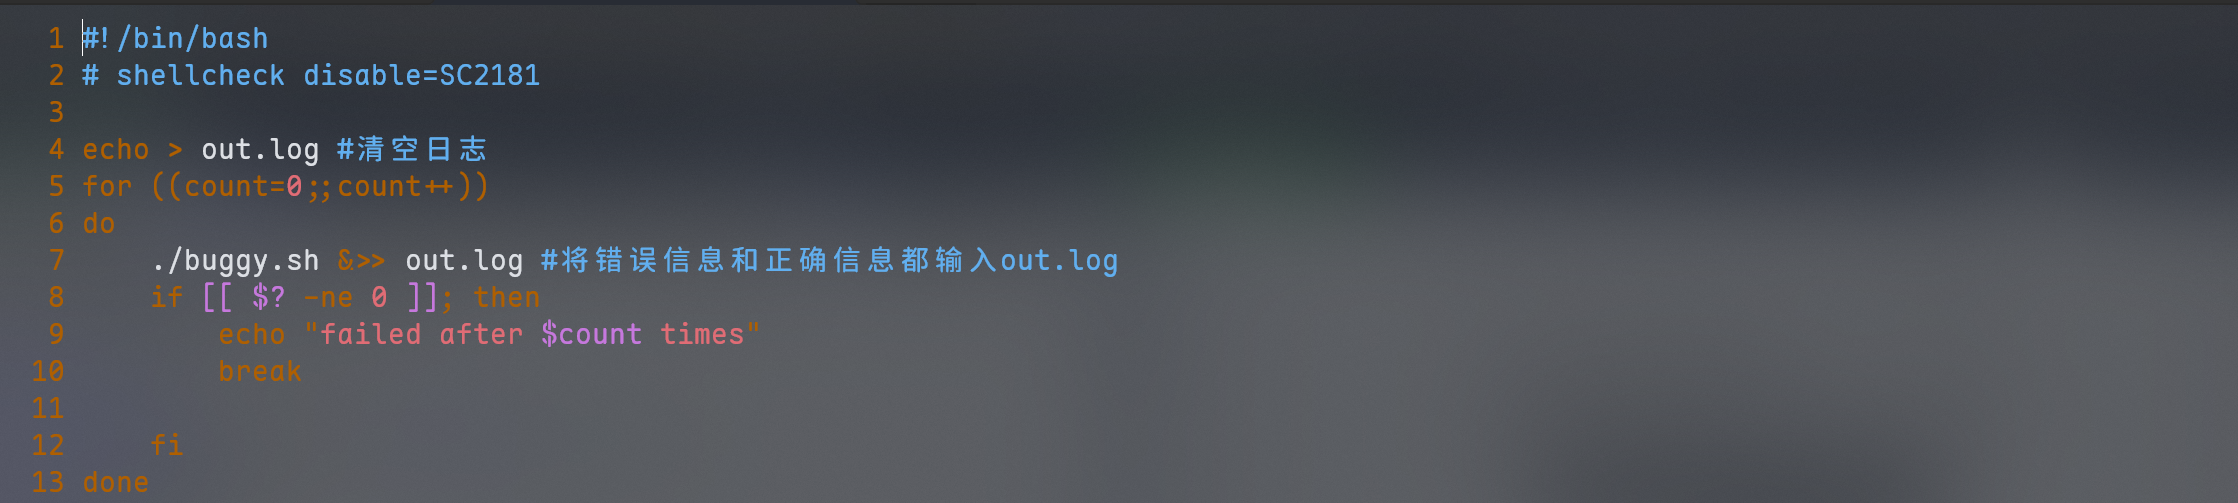
\includegraphics[width=0.75\linewidth]{debug_1.png}
    \caption{计数脚本}
    \label{fig:debug_1}
\end{figure}

\subsection{查找文件夹内某一类型的文件并进行压缩}
\begin{figure}[htb]
    \centering
    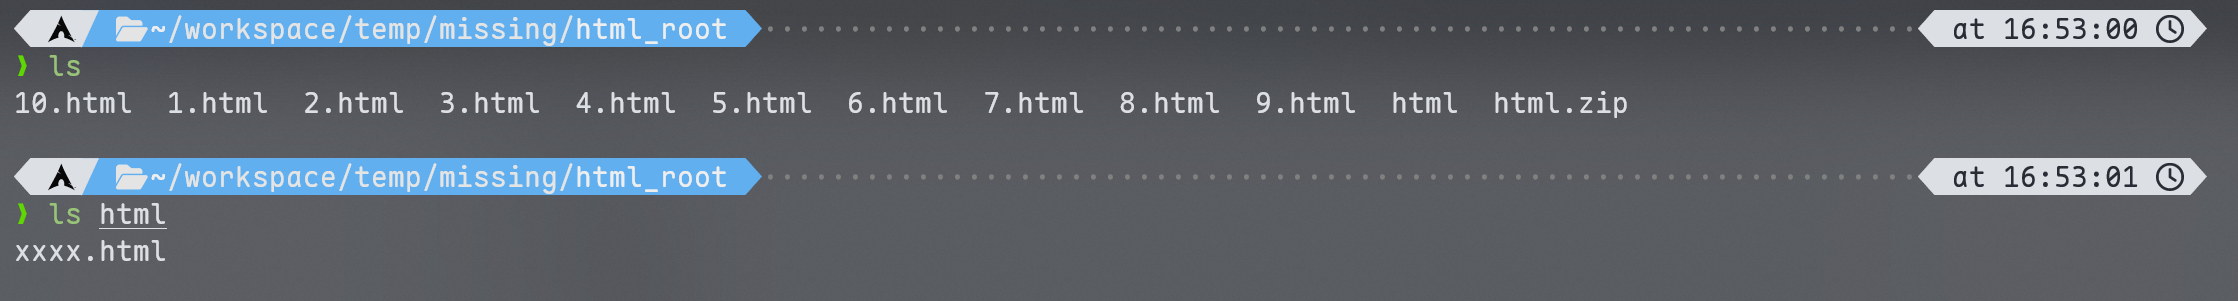
\includegraphics[width=0.75\linewidth]{html_1.png}
    \caption{原有文件}
    \label{fig:html_1}
\end{figure}
对文件夹内的html文件进行压缩,使用以下的命令:
\begin{figure}[htb]
    \centering
    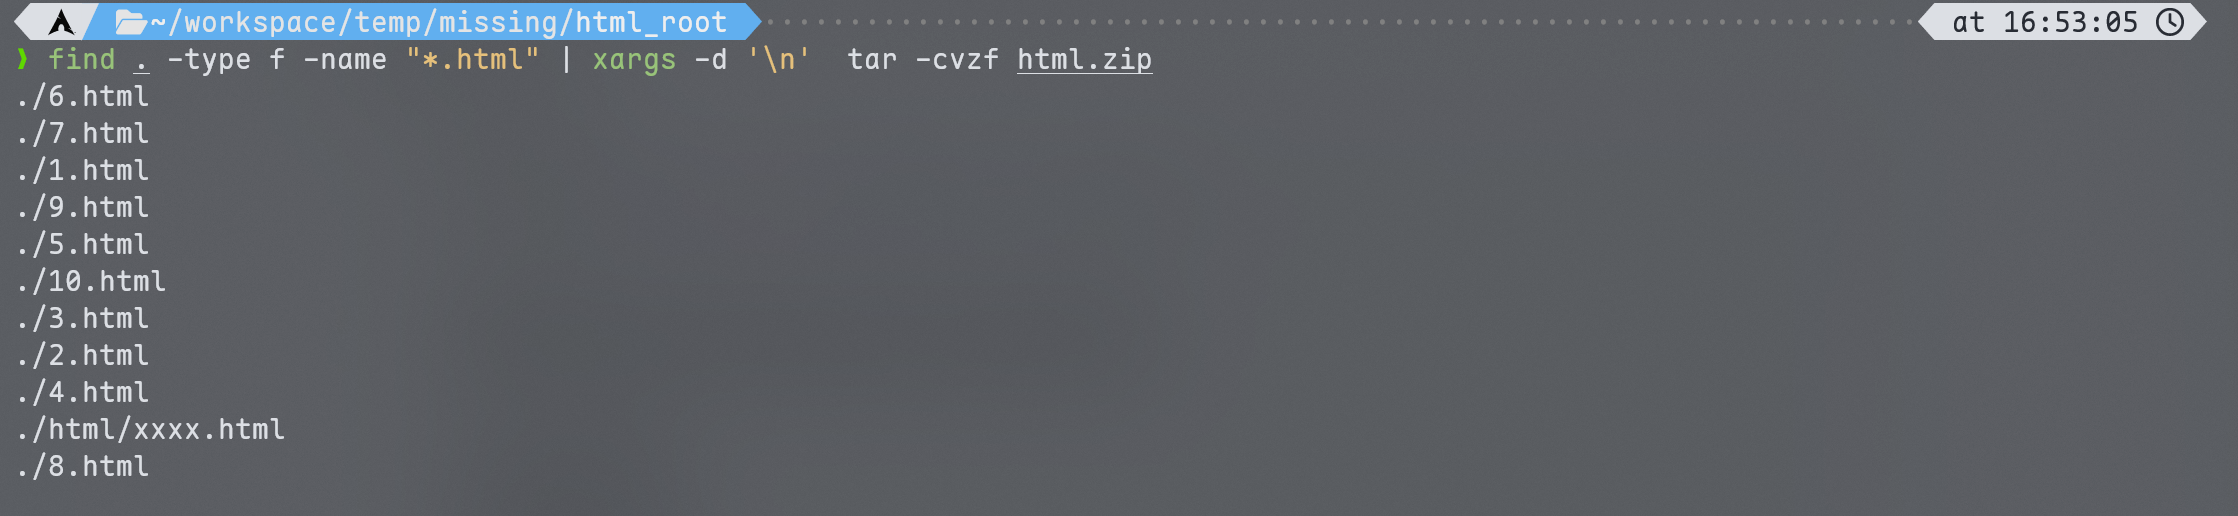
\includegraphics[width=0.75\linewidth]{tar_1.png}
    \caption{压缩命令}
    \label{fig:tar_1}
\end{figure}

.表示在当前目录下进行搜索,-type f指定搜索类型为文件,-name "*.html"代表搜索后缀名为html的文件,xargs将find搜索到的文件名以\verb|\n|分割,作为参数给tar,tar的-v表示将压缩的信息显示出来。

\subsection{移动文件或重命名文件}
移动文件:\mintinline{shell}|mv|。其衍生用法是对文件名进行修改,因为在移动文件时能顺带对其名称进行修改。不过要注意的是新文件名不能存在,否则就可能覆盖那个文件。
\begin{figure}[htb]
    \centering
    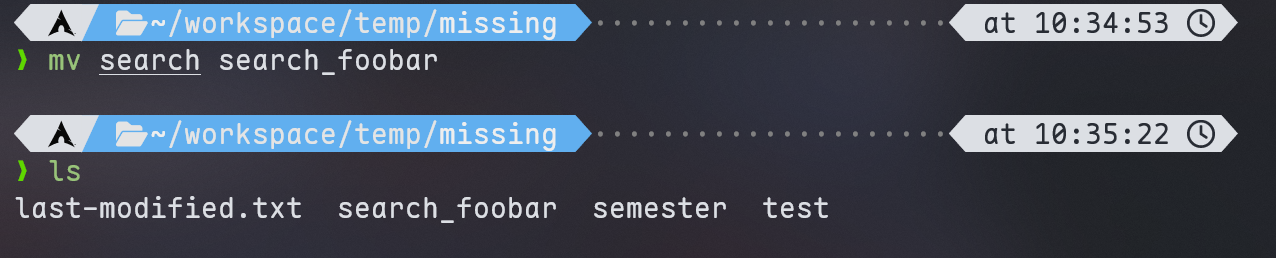
\includegraphics[width=0.75\linewidth]{mv_1.png}
    \caption{修改文件名}
    \label{fig:mv_1}
\end{figure}

\subsection{查看软件位置}
用于查找软件的目录,源代码或是手册页的位置。当需要知道Python解释器的路径以添加至Python脚本的shebang行时,whereis命令能帮上大忙。当解释器的路径被添加至shebang行后,就能直接通过\mintinline{shell}|./<script name>|来直接运行脚本,而不用添加 Python3 。

\subsection{查看历史命令,操作缓冲区,执行重复命令}
输入\mintinline{shell}|history|可以看到历史命令。使用Linux时输入的命令都储存在缓冲区中,\mintinline{shell}|history|能访问缓冲区并列出这些命令,可以使用\mintinline{shell}|history -w|保存缓冲区至.bash\_history文件,或使用\mintinline{shell}|history -c|清除缓冲区。
因为有缓冲区的存在,使得能够重复执行之前的命令,甚至指定执行某条历史命令。\mintinline{shell}|!!|能执行上一条命令,\mintinline{shell}|!N|可以执行第N条命令。还可以使用模糊匹配,\mintinline{shell}|!<command>:p|可以再次执行过去的命令。

还可以与grep配合,搜索与某个关键词匹配的命令。
\begin{figure}[htb]
    \centering
    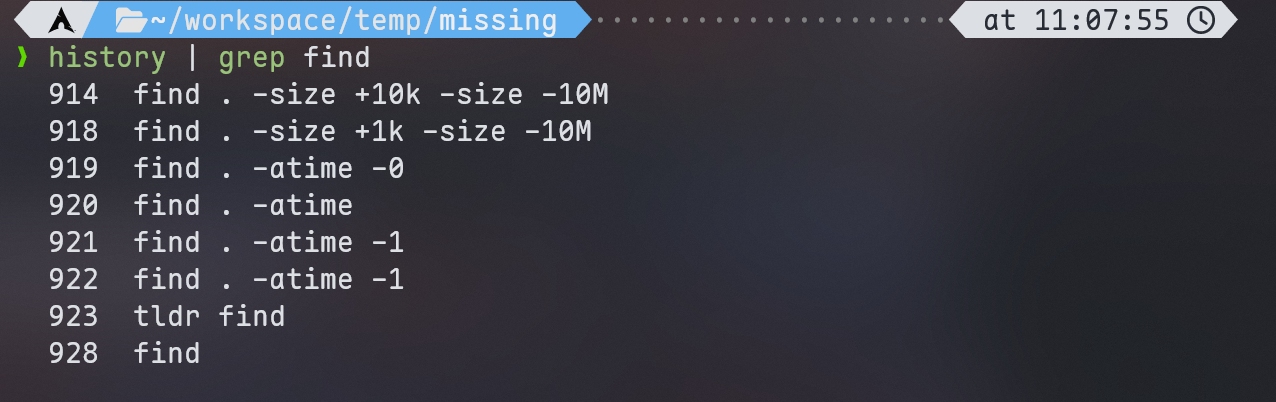
\includegraphics[width=0.75\linewidth]{history_1.png}
    \caption{history}
    \label{fig:history_1}
\end{figure}

\subsection{自定义shell}
zsh相对于bash是更优的shell选择,先修改默认shell为zsh。下载zsh并设置为默认shell,完成后一定要重新登录,才会看到shell为zsh。
\begin{listing}[htb]
    \begin{minted}{shell}
    安装zsh:sudo pacman -S zsh
    列出已安装的shell路径:sudo chsh -l
    修改默认shell:sudo chsh --shell <path to shell>
    \end{minted}
\end{listing}

接下来就是对zsh的自定义了。首先是安装Powerlevel10k,一个zsh主题,能够显示许多有用的信息,使用以下命令进行安装:
\begin{listing}[htb]
    \begin{minted}{shell}
    yay -S --noconfirm zsh-theme-powerlevel10k-git
    echo 'source /usr/share/zsh-theme-powerlevel10k/powerlevel10k.
    zsh-theme' >>~/.zshrc
    \end{minted}
\end{listing}

接着安装自动补全插件zsh-autosuggestions和快速导航插件autojump。
自动补全插件能显示推测的命令,通过右方向键接受建议,能大大提升命令效率。快速导航插件能根据子文件名进行导航,不需要输入完整路径。不过autojump很久未更新了,可能有一些问题。
\begin{listing}[htb]
    \begin{minted}{shell}
    sudo pacman -S zsh-autosuggestions
    git clone git://github.com/wting/autojump.git
    cd autojump
    ./install.py or ./uninstall.py
    \end{minted}
\end{listing}

\section{Vim学习感悟}
Vim的使用方式往往让初学者感到疑惑,插入文字还要进入特定的模式,退出还要输入特定的指令,而不会快捷跳转就只能用方向键一个字母一个字母地移动。

使用Vim最重要的是记住那些基本的按键,像快捷跳转,块选中。有了这些基本的按键,在文档中导航也变得更快捷,省去了移动鼠标的操作。像直接跳到文档末尾的操作,只要在Normal下按G就能实现,在Word中可没这么简洁。

配合tmux这样的终端复用器,在用Vim写代码时就能做到修改后马上看到运行效果,不需要再退出Vim后再运行,可以大大提升效率。
\begin{figure}[htb]
    \centering
    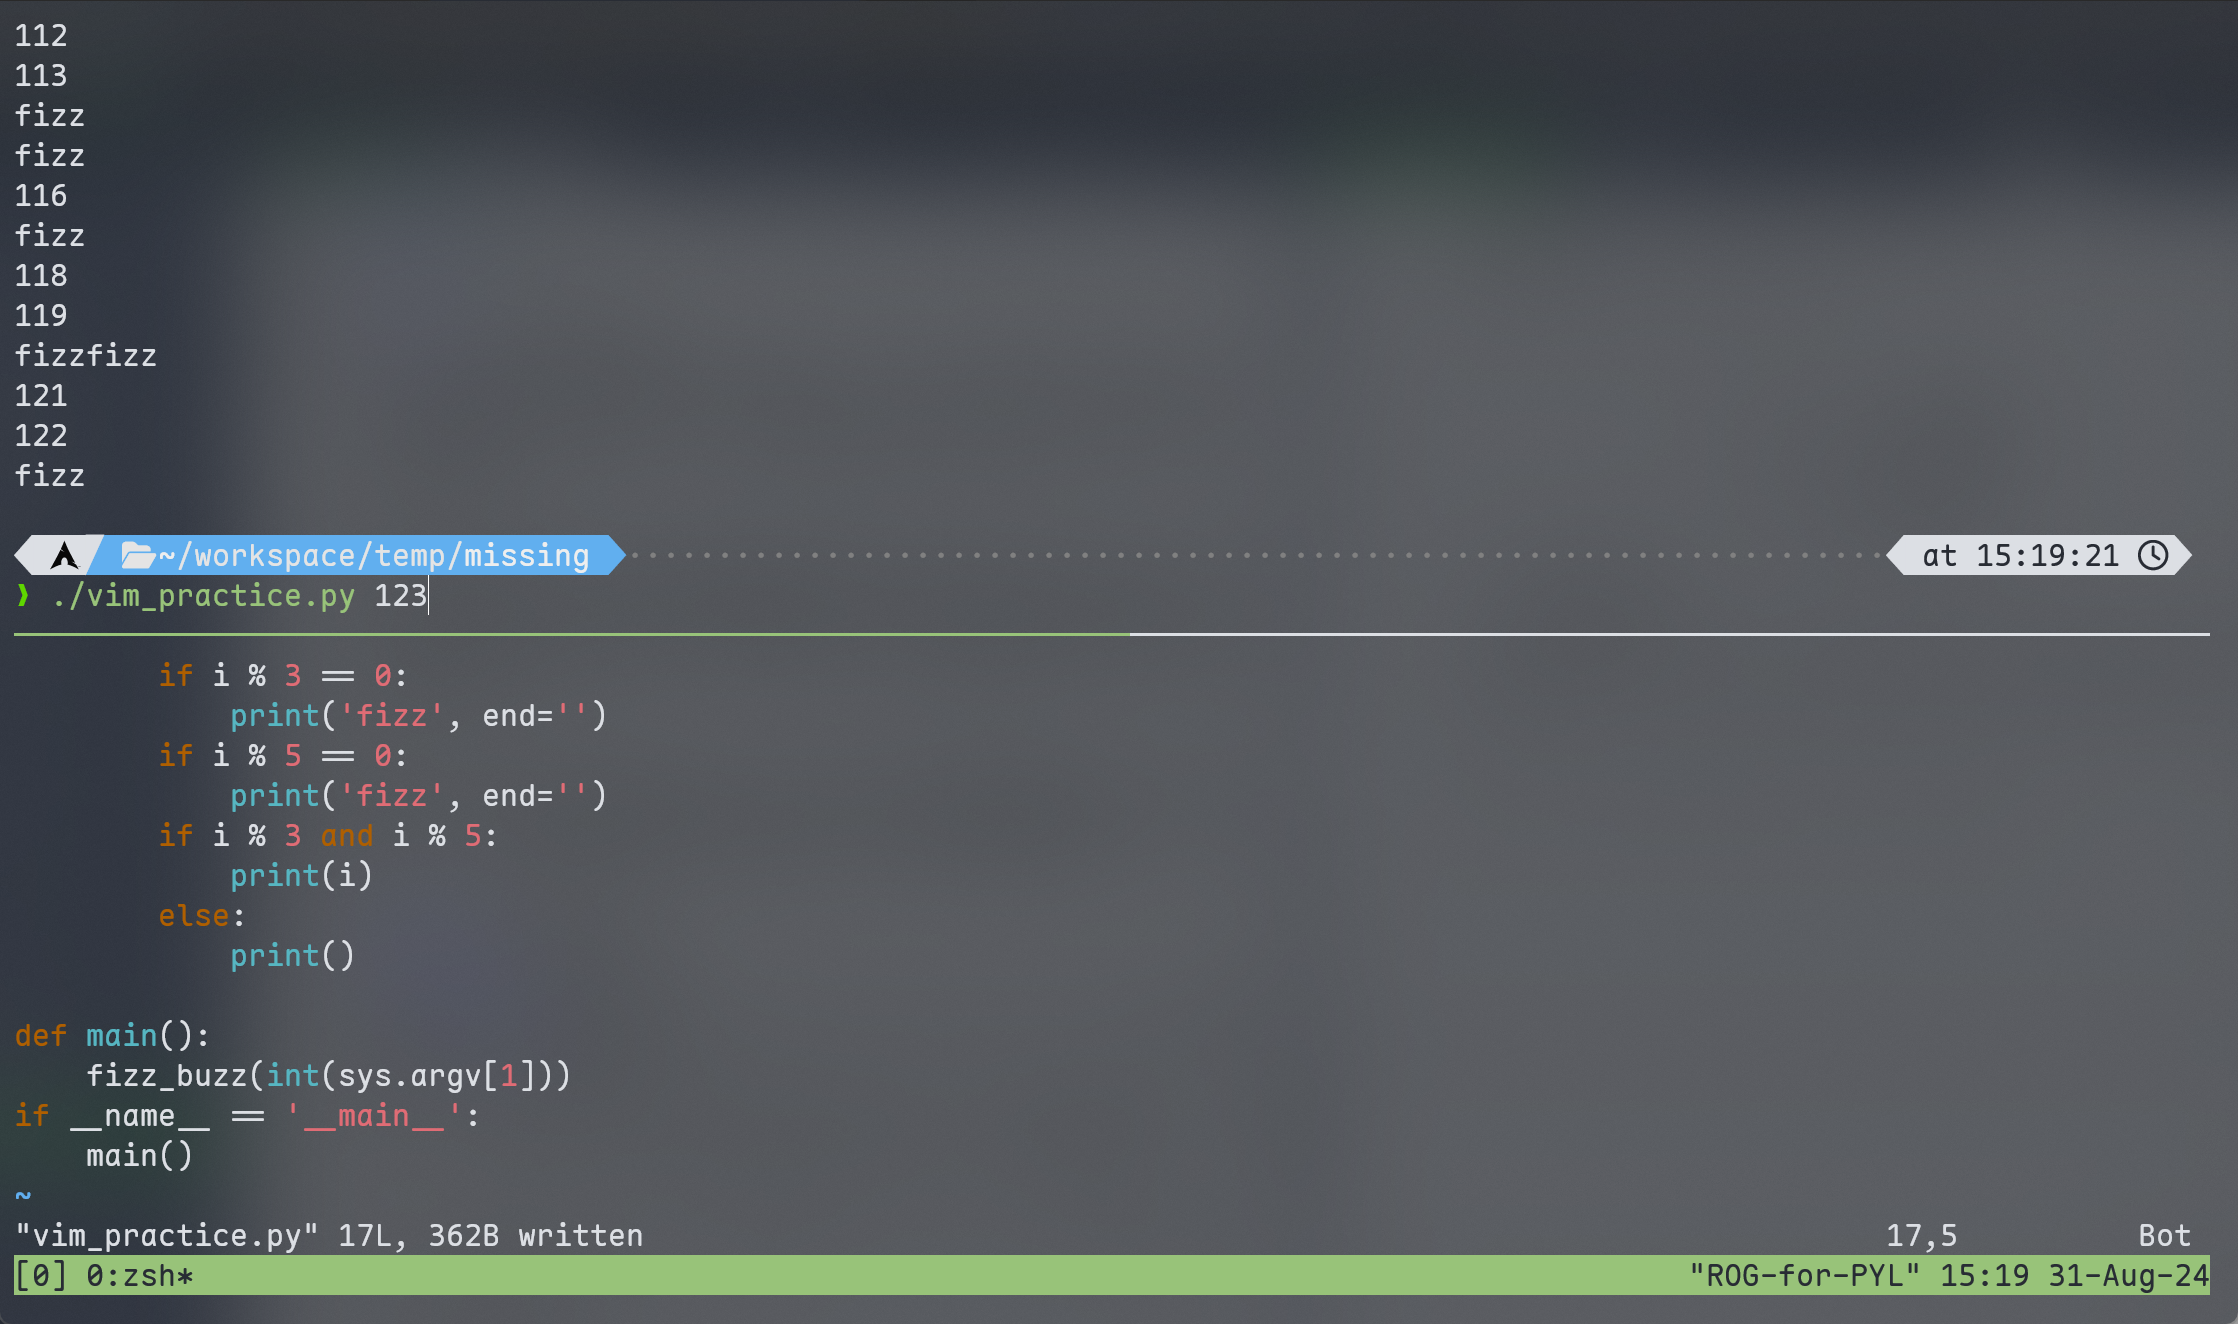
\includegraphics[width=0.75\linewidth]{vim_1.png}
    \caption{Vim配合tmux}
    \label{fig:vim_1}
\end{figure}

Vim也支持大量的自定义,可以修改下方的状态栏,显示更多的信息,也可以使用不同的主题,还可以安装自动补全插件,获得代码提示。

要注意的是Vim与系统的剪贴板互通需要一定的配置,在未配置前系统剪贴板的内容无法被Vim读取。

\section{Vim知识点}
\subsection{不同的模式}
使用\mintinline{shell}|vim|进入文件时,处于Normal 模式,可以通过不同的命令进入不同的模式。
键入 i 进入Insert 模式,R 进入Replace 模式,v 进入Visual 模式,V 进入Visual Line 模式,Ctrl-V进入Visual Block 模式,: 进入命令模式。

在wsl Ctrl-V中会与Windows的粘贴冲突,可以在.vimrc文件中的修改键位,\mintinline{javascript}|nmap <C-K> <C-v>|。

在Visual及类似模式中,可以移动光标选中内容,使用 y 复制选中内容,x 进行剪切,p 进行粘贴。

\subsection{快捷移动操作}
\subsubsection{全文件范围内}
在Normal模式下,gg移动到文件开头,G移动到文件末尾行的第一个非空格字符处。

\subsubsection{窗口范围内}
H,M,L分别移动到窗口的顶部,中部,底部。Ctrl-u向上滚动,Ctrl-d向下滚动。

\subsubsection{行范围内}
0移动到本行的开头,\$移动到本行的末尾,\^移动到本行首个非空格字符处。w移动到下一个词的开头,b移动到词的开头,e移动到词的末尾。

\subsection{快速新建行}
使用o在光标所在的下一行进行输入,O在光标所在的上一行进行输入。

\subsection{复制粘贴操作}
yy复制当前行,y0复制本行开头至游标的内容,y\$复制到本行末尾。
p粘贴至下一行,P粘贴至上一行。

\subsection{删除操作}
x删除光标后的字符,X删除光标前的字符。
dl删除光标后的字符,dh删除光标前的字符,0、\$也有类似y的效果。
dd删除本行,在文件开头使用dG可以删除整个文件的内容。但是这些删除操作都类似剪切,会将删除的内容存至剪贴板。

\subsection{撤销操作}
在Normal模式下,使用u可以撤销上一次保存后的所有操作,U撤销对某一行的全部操作,但是只能撤销本次打开文件以来所做的修改。

Ctrl-r能重做操作。

\subsection{命令行模式}
命令行模式用于文件的保存与打开、关闭。
\begin{itemize}
    \item \mintinline{shell}|:q| 退出Vim
    \item \mintinline{shell}|:w| 保存修改
    \item \mintinline{shell}|:wq| 保存修改并退出
    \item \mintinline{shell}|:e <filename>| 打开文件
    \item \mintinline{shell}|:ls| 列出打开的文件缓冲区
\end{itemize}

\subsection{编辑.vimrc进行自定义}
.vimrc是Vim的配置文件,放在HOME文件夹处,没有的话可以创建一个。.vimrc的注释符号是\mintinline{javascript}|"|。
以下是我的自定义,还没有添加插件:
\begin{figure}[htb]
    \centering
    \includegraphics[width=0.75\linewidth]{.vimrc_1.png}
    \caption{配置文件}
    \label{fig:.vimrc_1}
\end{figure}

\section{数据整理学习感悟}
个人感觉课程中所至的数据整理就是对信息进行筛查,课程中包含了\mintinline{shell}|grep less sed sort|还有正则表达式的使用,比较抽象,而且正则表达式的部分比较复杂,不太好理解。不过\mintinline{shell}|grep less sort|等命令在平时也能使用,还是很有帮助的。

\section{数据整理知识点}
\subsection{查看日志}
\mintinline{shell}|journalct|命令能够显示日志,配合\mintinline{shell}|less|能让输出的日志像文件一样可以翻页,再使用\mintinline{shell}|grep|就能抓取某些特定的信息。

\subsection{\mintinline{shell}|less|的使用}
可以用于查看文件,也可以查看标准输出流。在查看页面按q退出,空格和b进行上下翻页,G前往文件末尾,g前往文件开头,同样支持搜索文件。

\subsection{正则表达式}
通常以\verb|\|开始和结束,有一些字符代表特殊的含义,常见的有:
\begin{itemize}
    \item . 匹配除换行符之外的 “任意单个字符”
    \item * 匹配*前字符零次或多次
    \item + 匹配+前字符一次或多次
\end{itemize}
这是关于正则表达式的说明:\url{https://regexone.com/}。
在\mintinline{shell}|sed|中,通过使用正则表达式能够筛选出满足需要的字符,比如获取登录者的用户名。
\begin{figure}[htb]
    \centering
    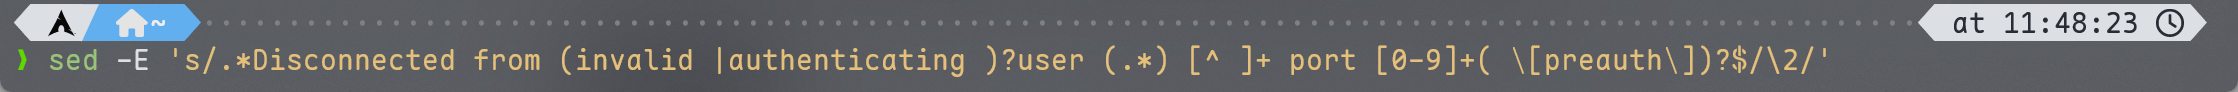
\includegraphics[width=0.75\linewidth]{sed_1.png}
    \caption{获取登录者的用户名}
    \label{fig:sed_1}
\end{figure}

\subsection{对数据排序}
\mintinline{shell}|sort|能对输入的数据进行排序,\mintinline{shell}|uniq -c|命令会把连续出现的行折叠为一行并用出现次数作为前缀,\mintinline{shell}|sort -n|命令能按数字顺序对输入进行排序,\mintinline{shell}|sort -k1,1|表示基于空格分割的第一列进行排序。在这一系列命令后就能过滤出最常出现的数据。

\end{sloppypar}
\end{document}